\documentclass[german]{book}
%\usepackage{url}
\PassOptionsToPackage{hyphens}{url}\usepackage[breaklinks=true]{hyperref}
\usepackage{dsfont}
\usepackage{listings}
\usepackage{german}
\usepackage[utf8]{inputenc}
\usepackage[final]{graphicx}

\begin{document}

\title{Open Historical Data Map\\
Systembeschreibung \\
Version 0.0.0
}

\author{
Thomas Schwotzer \\
Mohamadbehzad Karimi Ahmadabadi\\
Daniel Schulz\\
nächste/r Projektleiter/in\\
(Herausgeber)
}

\maketitle

\tableofcontents

\chapter{Überblick}
\section{Dokumentengeschichte}
\begin{table}[h]
 \begin{tabular}{|l|l|p{4cm}|}
 \hline
 Zeitraum & PL/Autor(en) & Änderungen \\
 \hline
 Sommersemester 1980 & IHR NAME & 
text \newline 
text \newline 
text \newline 
text \newline 
text \newline 
text \newline 
 
  \\
 \hline
 Wintersemester 1980/81 & IHR NAME & 
text \newline 
text \newline 
text \newline 
text \newline 
text \newline 
text \newline 
 
  \\
 \hline
 
 
 \end{tabular}
 \caption{Dokumentengeschichte}
 \end{table}

\section{Ziel des Systems}
\section{Laufenden Arbeiten}
\section{Pläne}


\chapter{OHDM-Datenmodell}
\section{Dokumentengeschichte}
\begin{table}[h]
 \begin{tabular}{|l|l|p{4cm}|}
 \hline
 Zeitraum & PL/Autor(en) & Änderungen \\
 \hline
 Sommersemester 1980 & IHR NAME & 
text \newline 
text \newline 
text \newline 
text \newline 
text \newline 
text \newline 
 
  \\
 \hline
 Wintersemester 2017/18 & Behzad Karimi & 
Bild eingefügt (Bilder ab jetzt mit 120mm einfügen) \newline 
text \newline 
text \newline 
text \newline 
text \newline 
text \newline 
 
  \\
 \hline
 \end{tabular}
 \caption{Dokumentengeschichte}
 \end{table}

\section{Aufgabe der Komponente}
%\begin{figure}[h!]
%\centering
%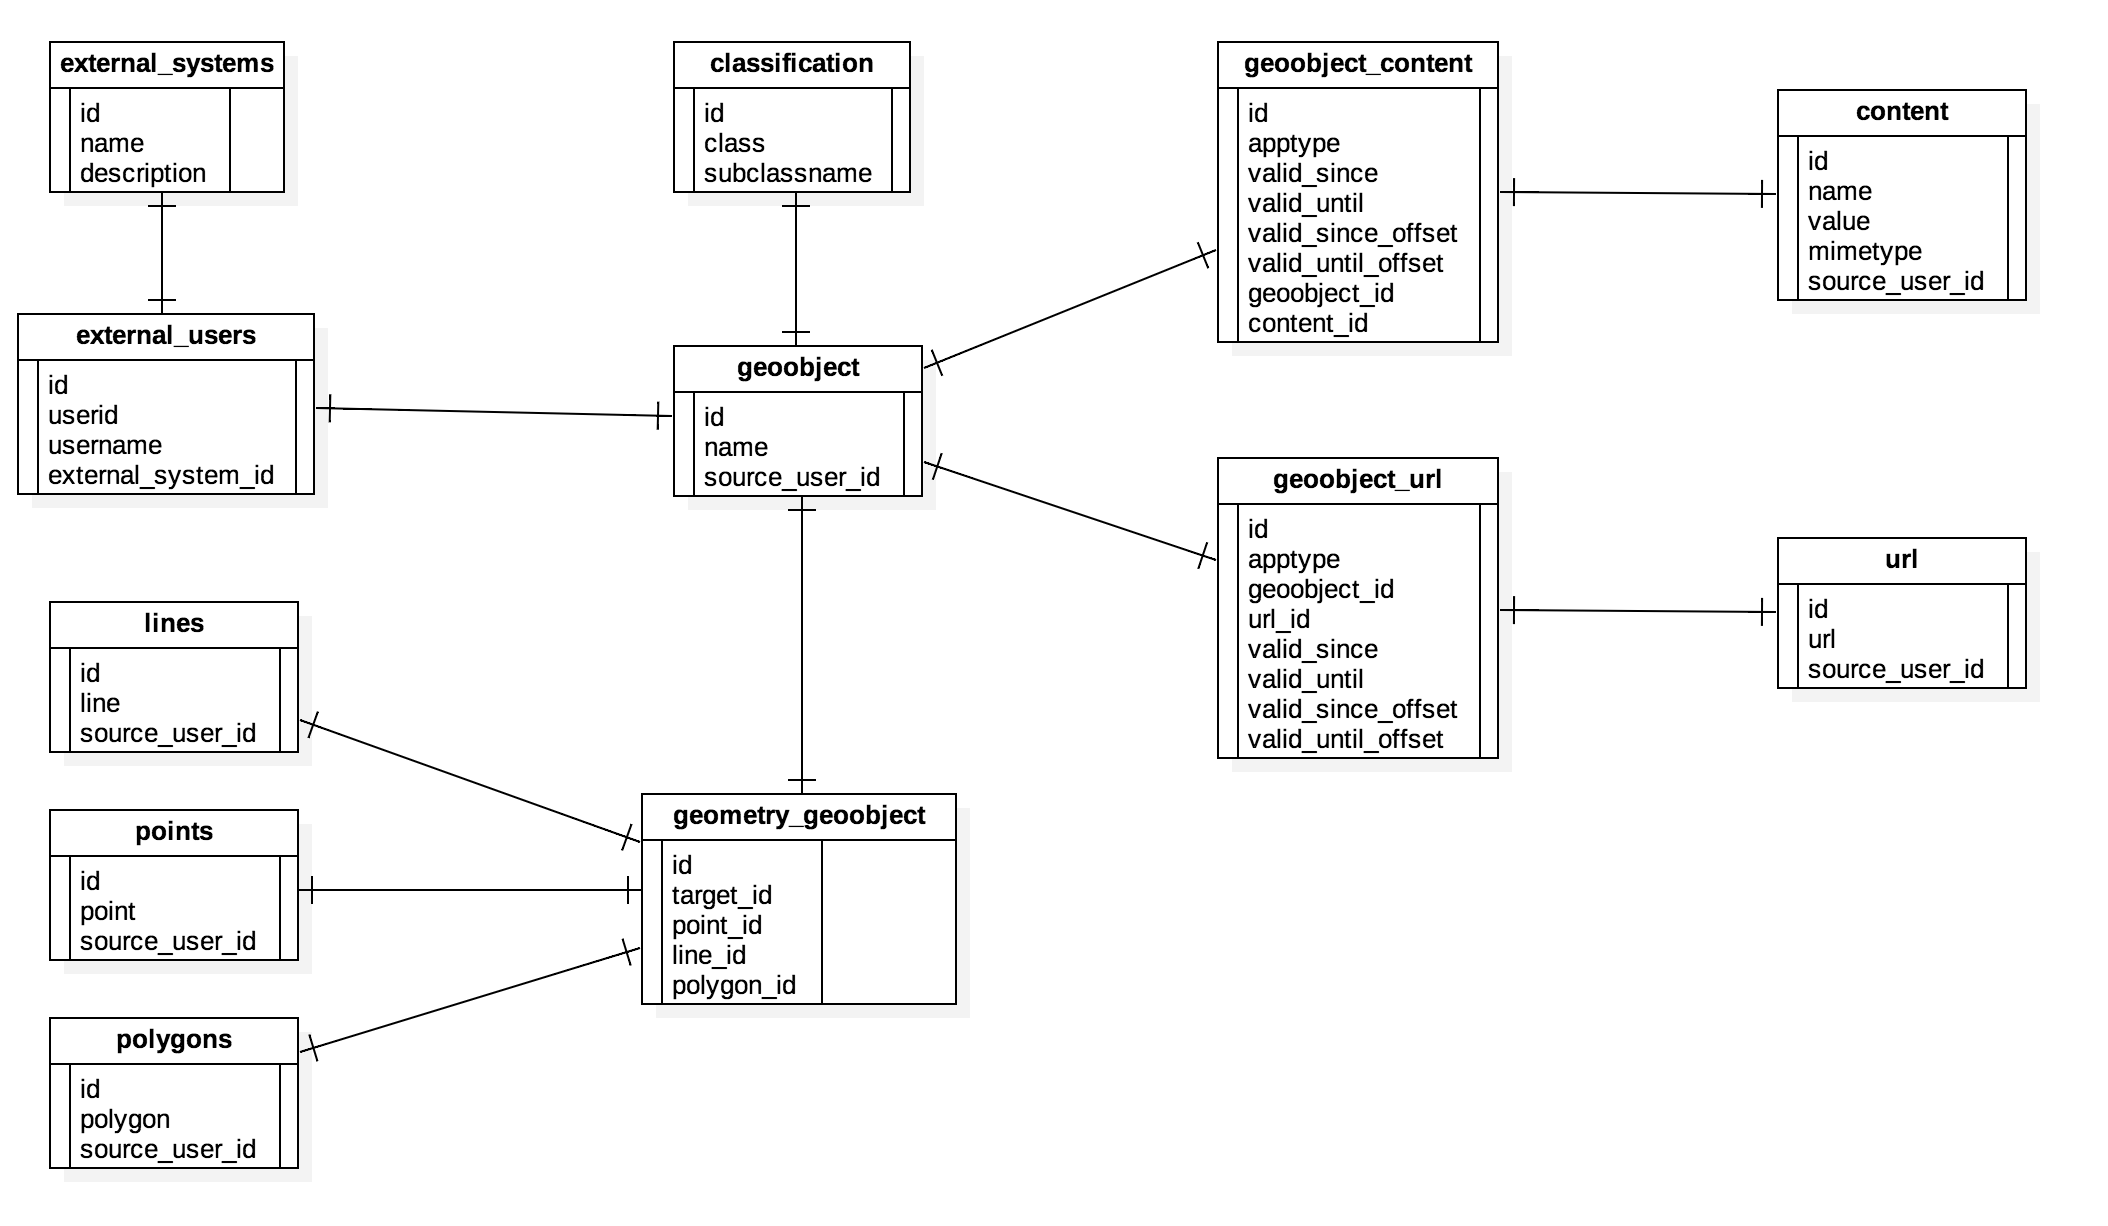
\includegraphics[width=127mm]{ohdm_datenmodell/ohdm_data_modell.png}
%\caption{OHDM Datamodell}

%\label{fig:datamodell}
%\end{figure}


Im Datenmodell von OHDM geht alles vom Geoobjekt (geoobject) aus. Dieses zentrale Object beschreibt alle Modelle auf der Karte, da alle Informationen der Modelle auf das geobject verweisen. Das einzige Objekt worauf das geobject verweist, ist der Ersteller (external\_users). Der Ersteller des Objekts greift durch ein externes System (external\_systems) auf dern Server zu und gibt die Informationen über das Geobjekt weiter. Wie nun ein Geobjekt im Allgemeinen aussieht wird im nächsten Abschnitt beschrieben.

\subsection{Geometrien in GIS}
Da OHDM mit PostGIS arbeitet (für GIS siehe ...) werden die zweidimensionalen Objekte als Polygone repräsentiert. Polygone bestehen dabei aus Punkten (points) und Linien (lines). Die Punkte werden mit Linien verbunden, so dass am Ende ein Polygon entsteht. Der folgende Satz ist dabei eine Vorraussetzung für einen Polygon:
\begin{center}
 \textit{Ein Polygon, eine geoordete Menge von Strecken, mit der Eigenschaft, dass ein Punkt der letzten Strecke identisch zu einem Punkt der ersten Strecke ist.}
 \end{center} 
Das heißt ein Polygon kann ohne Punkte und Linien nicht existieren. Ebenso kann eine Linie ohne zwei Punkte nicht existieren. Wie erstellt man nun ein Gebäudekomplex aus mehreren Gebäuden? Diese sogenannten \textit{Multi-Polygone}, sind mehrere nicht überlappende Polygone. Dann gibt es noch die Möglichkeit Löcher in den Polygonen zu erstellen. Diese Löcher sind nichts weiter als ein Polygon in einem anderen Polygon. In GIS gibt es dabei folgende Einschränkungen:
\begin{itemize}
\item Polygone im inneren dürfen sich untereinander nicht überlappen. Falls doch, könnten sie auch als ein einzelnes Polygon dargestellt werden.
\item Ein Rand eines inneren Polygons darf nicht Rand des äußeren Polygons sein. Falls dem nämlich so ist, wird das äußere Polygon nämlich anders dargestellt werden. %TODO @Behzad wie dargestellt?
\item Aus dem oberen Satz lässti sich auch folgende Eigenschaft erklären. Kein Punkt des inneren Polygons darf gleichzeitig dem äußerem Polygon gehören. Hier würden ebenfalls das äußere Polygon ansonsten anders dargestellt werden. %TODO @Behzad auch hier, wie?
\end{itemize}
%TODO 
Wie genau nun Objekte enstehen und Polygone dargestellt werden, wird im Kapitel ( ...TODO... ) genauer erläutert. Damit die Polygone bzw. Geobjekte ordentlich auf der Karte  dargestellt werden können, teilem wir jedem Geoobjekt eine Klasse (class) zu. 

\subsection{Klassifikation von Geoobjekten}
Die Entity classification weißt mit einer ID auf das Geoobjekt hin und teilt diesen in eine bestimmte Klasse ein. Jede Klasse hat wiederum nochmals Unterklassen. Dadurch können wir Geoobjekte genau beschreiben um diese auf der Karte dementsprechend anzuzeigen. Zu Klassen gehört zum Beispiel: Geschäft, Gebäude, Autobahn, Büro, historisch, Tourismus, etc.. Zu den Unterklassen gehören Dinge wie: Bahnhof, Flugplatz, Fahrrad, Brücke, Busstaion, etc.. %TODO @Behzad den Unterschied bitte genauer erklären, bin noch etwas verwirrt
Nun können wir Geoobjekte darstellen und erklären zu welcher Klasse bzw. Unterklasse diese gehören. Wie nun genau ein Polygon dargestellt wird, erklären wir im nächsten Abschnitt.

\subsection{Der Inhalt eines Geoobjekts}
Die Entity geoobject\_content verweist anhand einer ID auf die Instanz Inhalt (content). Dort wird beschrieben was genau das Geoobjekt ist. Wenn z.B. auf einer Karte die HTW zu erkennen ist und darauf geklickt wird, werden Informationen angezeigt die in dieser Instanz gespeichert sind. Zurück zur Instanz geoobject\_content. Dort werden Zeitliche Informationen gespeichert, wie z.B. bis wann das Objekt existierte. 
Wir möchten nun in OHDM eine Möglichkeit haben, anhand einer URL auf spezifische Geoobjekte zuzugreifen. Damit das möglich ist gibt es zwei weitere Instanzen.

\subsection{URLs für Geoobjekte}
In der Instanz URL (url) existiert eine URL womit direkt auf das verwiesene Geobjekt zugegriffen werden kann. Diese Instanz weist aber erst auf die Instanz geoobject\_url welche denselben Inhalte wie die Insatnz geoobject\_content speichert.
%TODO @Behzad warum gibt es geoobject_content und geoobject_url wenn beide fast dieselben Attribute haben? warum nicht in eine Tabelle speichern? 

\section{Architektur}

\subsection{Überlick}
Grafik der Teile der Komponente (wichtig: Benennung aller Schnittstellen). 
Anwendung der Komponente nennen (Use Case).

Übliche Interaktionen durch Interaktionsdiagramme.

(Ausfüllen in Prototyp-Phase)

\subsection{Schnittstellendefinitionen}
Beschreibung der angebotenen Schnittstellen. Benennung der Funktionen
mit Vor- und Nachbedingungen. Beschreibuung des Protocol-Bindings.

(Beginnen in Prototyp-Phase. Konkretisieren in der Alphaphase)

\subsection{genutztes Komponenten}
Beschreibung, welche weiteren Komponenten (in welchen Versionen, wo beziehbar) genutzt werden.

(Beginnen in Prototyp-Phase. Konkretisieren in der Alphaphase)

\section{Nutzung}
\subsection{Code}
Wo findet man den Code. Struktur des Codes. (In Prototyphase ausfüllen,
kann dort sehr kurz sein. Ab Alpha-Phase konkret beschreiben.)

\subsection{Deployment / Runtime}
Beschreibung wie die Komponenten aus dem Quellcode erzeugt werden kann,
wie sie installiert wird und wie man sie startet.

\section{Qualitätssicherung}
(Ausfüllen ab Alpha-Phase).

Wie erfolgt die Sicherung der Qualität? Keine Romane, sondern ehrlich notieren,
was man tut. Wenn man nichts tut, dann steht hier: Wir sichern die Qualität der
Komponente nicht.

Issue-Tracking: wie erfolgt das, interne Fehlermeldungen (ab Alpha), 
externe Fehlermeldungen ab Beta.

\subsection{Test}
Wie wird die Komponente getestet.

\section{Vorschläge / Ausblick}
Was ist aufgefallen, was sollte man ändern? Löschen Sie auch gern die Kommentare
der Vorgänger, aber nur, wenn es wirklich nicht mehr relevant ist.



\chapter{Kartenerzeugung und WMS/WFS}
\section{Dokumentengeschichte}
\begin{table}[h]
 \begin{tabular}{|l|l|p{4cm}|}
 \hline
 Zeitraum & PL/Autor(en) & Änderungen \\
 \hline
 Sommersemester 1980 & IHR NAME & 
text \newline 
text \newline 
text \newline 
text \newline 
text \newline 
text \newline 
 
  \\
 \hline
 Wintersemester 1980/81 & IHR NAME & 
text \newline 
text \newline 
text \newline 
text \newline 
text \newline 
text \newline 
 
  \\
 \hline
 \end{tabular}
 \caption{Dokumentengeschichte}
 \end{table}

\section{Aufgabe der Komponente}
Verbale kurze prägnante Beschreibung, was die Komponente leisten soll.
Das sind wenige Seiten.

(Ausfüllen in Prototyp-Phase)

\section{Architektur}

\subsection{Überlick}
Grafik der Teile der Komponente (wichtig: Benennung aller Schnittstellen). 
Anwendung der Komponente nennen (Use Case).

Übliche Interaktionen durch Interaktionsdiagramme.

(Ausfüllen in Prototyp-Phase)

\subsection{Schnittstellendefinitionen}
Beschreibung der angebotenen Schnittstellen. Benennung der Funktionen
mit Vor- und Nachbedingungen. Beschreibuung des Protocol-Bindings.

(Beginnen in Prototyp-Phase. Konkretisieren in der Alphaphase)

\subsection{genutztes Komponenten}
Beschreibung, welche weiteren Komponenten (in welchen Versionen, wo beziehbar) genutzt werden.

(Beginnen in Prototyp-Phase. Konkretisieren in der Alphaphase)

\section{Nutzung}
\subsection{Code}
Wo findet man den Code. Struktur des Codes. (In Prototyphase ausfüllen,
kann dort sehr kurz sein. Ab Alpha-Phase konkret beschreiben.)

\subsection{Deployment / Runtime}
Beschreibung wie die Komponenten aus dem Quellcode erzeugt werden kann,
wie sie installiert wird und wie man sie startet.

\section{Qualitätssicherung}
(Ausfüllen ab Alpha-Phase).

Wie erfolgt die Sicherung der Qualität? Keine Romane, sondern ehrlich notieren,
was man tut. Wenn man nichts tut, dann steht hier: Wir sichern die Qualität der
Komponente nicht.

Issue-Tracking: wie erfolgt das, interne Fehlermeldungen (ab Alpha), 
externe Fehlermeldungen ab Beta.

\subsection{Test}
Wie wird die Komponente getestet.

\section{Vorschläge / Ausblick}
Was ist aufgefallen, was sollte man ändern? Löschen Sie auch gern die Kommentare
der Vorgänger, aber nur, wenn es wirklich nicht mehr relevant ist.



\chapter{OSM-Archiv}
\section{Dokumentengeschichte}
\begin{table}[h]
 \begin{tabular}{|l|l|p{4cm}|}
 \hline
 Zeitraum & PL/Autor(en) & Änderungen \\
 \hline
 Wintersemester & Schwotzer, Thomas & 
OSM parsen und Fülle Intermediate DB
   \\
 \hline
 Wintersemester 1980/81 & IHR NAME & 
text \newline 
text \newline 
text \newline 
text \newline 
text \newline 
text \newline 
 
  \\
 \hline
 \end{tabular}
 \caption{Dokumentengeschichte}
 \end{table}

\section{Aufgabe der Komponente}
Eine, wenn nicht die, wesentliche Quelle für OHDM ist Open Street 
Map (OSM)\footnote{osm.org}.

In einem {\it initialen Upload} wurde OHDM im Sommer 2017 mit
den Daten des Planet.osm Files vom Januar 2017 gefüllt.

Diese Komponenten realisiert daneben das jährlich Update der
OHDM Datenbank basierend auf OSM-Planet-Files.

Der Update-Prozess wird im Detail weiter unten beschrieben.

\section{Architektur}
Die Komponente teilt sich in zwei Subkomponenten:

\begin{description}
\item[OSM2Intermediate] 
parsed das OSM File und füllt die
Intermediate Database.

\item[Intermediate2OHDM] füllt oder erneuert die OHDM Datenbank 
mit Daten aus OSM.

\end{description}

Diese Komponenten bietet keine Schnittstelle nach außen an.

Diese Komponente nutzt keine weiteren Komponenten des Systems.

\section{OSM-to-Intermediate}
Diese Teilkomponenten parsed die OSM Files und füllt die Intermediate Database.
Die Struktur der Intermediate ist einfach. Sie enthält fünf Tabellen.

Die Tabelle {\tt nodes}, {\tt ways} und {\tt relations} werden direkt aus
den Einträgen im OSM-File gefüllt. Jede Tabelle enthält OSM-Nutzer und -ID.
Die Nodes enthalten die Koordinaten. Ways und Relations enthalten die IDs
der Nodes bzw. Ways, die den Way bzw. die Relation beschreiben.

Die IDs werden in diesen Tabelle als String gehalten. Dadurch wird die
Reihenfolge der IDs gespeichert.

Es gibt zwei weitere Tabelle: {\tt waynodes} repräsentiert die 1-n Beziehung
zwischen ways und nodes. Die {\tt relationsmember} speichert die 1-n-Beziehung 
zwischen Relation und ihren Membern (nodes bzw. ways.)

\subsection{SQL\_OSMImporter}
Der {\tt SQL\_OSMImporter} implementiert {\tt DefaultHandler} und arbeitet wie folgt:

\subsubsection{Begin / Ende Dokument}
Der Parser erkennt den Beginn und das Ende des XML Dokuments. Diese Events werden jeweils
einmal am Anfang und am Ende des Parse-Prozesses geworfen. Die Methoden {\tt startDocument()}
und {\tt endDocument()} werden dabei aufgerufen. Bei Beginn wird eine Statusmeldung erzeugt.

Am Ende werden die {\tt SQLQueues} geschlossen - siehe dazu \ref{SQLStatementQueue}.

\subsubsection{Start / End Element}
Der Parser ruft die Methode {\tt startElement()} auf, wenn er den Beginn eines XML
Tags erkennt. Die Methode {\tt endElement()} wird gerufen, wenn das Ende eines
XML Elements entdeckt wird. XMl-Elemente können geschachtelt sein und sind es im
OSM-XML-File auch. Einem Aufruf eines {\tt startElement()} können weitere Aufrufe
der gleichen Methode folgen, weshalb der Zustand relevant ist, in dem der Aufruf erfolgt.

Die beiden Methoden werden durch den Importer implementiert. Es gibt sechs verschiedene
Tags im OSM File. Die Tags {\tt node, way, relation} enthalten Beschreibungen von Punkten,
Wegen oder Relationen. Die Tags {\tt tag, nd, member} treten nur innerhalb der Tags
auf.

Die ersten drei Tags dürfen nur als direkte Kindknoten der XML-Root
auftauchen. Es wird deshalb geprüft, ob der Parser aktuell {\it außerhalb - OUTSIDE}
war, d.h. auf der Ebene der Root. Es ist ein Fehler, wenn das nicht der Fall ist.
Der Fehler wird aber ignoriert, was nicht sauber programmiert ist (!).

Im Erfolgsfall wird für {\tt node, way, relation} die Methode {\tt newElement} aufgerufen.
Im Fall von {\tt tag, nd, member} wird jeweils {\tt addAttributes, addND, und addMember} aufgerufen.

Das Tag {\tt tag} enthält weitere Informationen zu dem Element - das sind Attribute,
die später in die Intermediate DB eingetragen werden. Das Tag {\tt nd} gibt es nur innerhalb
von {\tt way} Tags. Es folgt die ID eines Nodes, das Teil des Weges ist. Das Tag {\tt member}
gibt es nur innerhalb einer {\tt relation}. Es folgen Beschreibungen (vor allem IDs)
der Member einer Relation. Das können Nodes und Ways sein.

\subsubsection{newElement}
Mit jedem Aufruf von {\tt newElement} wird ein {\tt INSERT} Kommando erzeugt.
Dieses Kommando wird nicht direkt an die Datenbank geschickt, sondern in einer 
{\tt SQLStatementQueue} gepuffert, siehe \ref{SQLStatementQueue}. Das dient lediglich
der Performance.

In dieser Implementierung werden parallel mehrere {\tt SQLStatementQueues} gefüllt.
Die Insert-Queue enthält {\tt INSERT}-Statements, die die Tabellen {\tt node, ways, relations}
der Intermediate DB füllen. Die Member-Queue sammelt Statements, die in die {\tt waynodes, relationmember}
gespeichert werden.

Der Code mag anfangs etwas verwirrend sein. Es hilft, zu verfolgen, wie die verschiedenen
Queues nacheinander gefüllt werden. Es ist auch zu beachten, dass die Statements erst mit
dem Aufruf von {\tt endElement} geschlossen werden. 

Es gilt auch zu beachten, dass zwischen den Start und dem Ende eines Elements auch
die anderen drei Methoden {\tt addAttributes, addND, und addMember} aufgerufen werden
können, die die {\tt INSERT}-Statement im weitere Parameter ergänzen.

\section{Utilities}
\subsection{SQLStatementQueue}
\label{SQLStatementQueue}
Objekte von {\tt SQLStatementQueue} sind ein Puffer zwischen dem Parser/Handler und
der Datenbank. Objekte der {\tt SQLStatementQueue} werden mit einem Parameterfile erzeugt.
In dem File stehen die wesentlichen Informationen, um eine JDBC-Connection zu einer Datenbank
zu erzeugen.

Danach arbeiten sie ähnlich einem {\tt StringBuilder}. Es können schrittweise mit {\tt append}
String hinzugefügt werden. Die Objekte prüfen nicht, ob eine gültige SQL-Syntax entsteht.
Die Objekte senden die Statement an die Datenbank, wenn ein definierbarer Schwellwert erreicht
ist oder wenn explizit die Methode {\tt force} (in Varianten) aufgerufen wird.

Eine Variante sind die FileSQLQueues. Diese erzeugen Files, in denen die Statements gespeichert
werden. Die Managed-Queues sorgen außerdem dafür, dass diese Files nach einem gewissen Füllstand
geschlossen werden und mittels psql ausgeführt werden. 

Die Implementierung dieser Klassen ist sehr stabil. {\bf Der Nutzung hat sich bewährt und ist in
dieser Komponente Pflicht!}

\section{Intermediate-to-OHDM}
Der Quellcode dieser Teilkomponenten liegt im package {\tt osm2inter}.

Das Package enthält nur wenige Klassen. {\tt OSMImport} enthält die {\tt main()}
Funktion. Dort wird ein {\tt SAXParser} erzeugt. Der Parser benötigt ein
Objekt, das die Klasse {\tt DefaultHandler} implementiert.

Der Parser parsed darauf das OSM-File. Sobald ein neues XML-Element gefunden wurde,
wird eine entsprechende Methode auf dem DefaultHandler aufgerufen. 

\section{Nutzung}
Der Code befindet sich im Repository {\tt OSMUpdateInsert}\footnote{https://github.com/OpenHistoricalDataMap/OSMImportUpdate}
\subsection{Code}
Wo findet man den Code. Struktur des Codes. (In Prototyphase ausfüllen,
kann dort sehr kurz sein. Ab Alpha-Phase konkret beschreiben.)

\subsection{Deployment / Runtime}
Beschreibung wie die Komponenten aus dem Quellcode erzeugt werden kann,
wie sie installiert wird und wie man sie startet.

\section{Qualitätssicherung}
(Ausfüllen ab Alpha-Phase).

Wie erfolgt die Sicherung der Qualität? Keine Romane, sondern ehrlich notieren,
was man tut. Wenn man nichts tut, dann steht hier: Wir sichern die Qualität der
Komponente nicht.

Issue-Tracking: wie erfolgt das, interne Fehlermeldungen (ab Alpha), 
externe Fehlermeldungen ab Beta.

\subsection{Test}
Wie wird die Komponente getestet.

\section{Vorschläge / Ausblick}
Was ist aufgefallen, was sollte man ändern? Löschen Sie auch gern die Kommentare
der Vorgänger, aber nur, wenn es wirklich nicht mehr relevant ist.



\chapter{Import}
\section{Dokumentengeschichte}
\begin{table}[h]
 \begin{tabular}{|l|l|p{4cm}|}
 \hline
 Zeitraum & PL/Autor(en) & Änderungen \\
 \hline
 Sommersemester 1980 & IHR NAME & 
text \newline 
text \newline 
text \newline 
text \newline 
text \newline 
text \newline 
 
  \\
 \hline
 Wintersemester 1980/81 & IHR NAME & 
text \newline 
text \newline 
text \newline 
text \newline 
text \newline 
text \newline 
 
  \\
 \hline
 \end{tabular}
 \caption{Dokumentengeschichte}
 \end{table}

\section{Aufgabe der Komponente}
Verbale kurze prägnante Beschreibung, was die Komponente leisten soll.
Das sind wenige Seiten.

(Ausfüllen in Prototyp-Phase)

\section{Architektur}

\subsection{Überlick}
Grafik der Teile der Komponente (wichtig: Benennung aller Schnittstellen). 
Anwendung der Komponente nennen (Use Case).

Übliche Interaktionen durch Interaktionsdiagramme.

(Ausfüllen in Prototyp-Phase)

\subsection{Schnittstellendefinitionen}
Beschreibung der angebotenen Schnittstellen. Benennung der Funktionen
mit Vor- und Nachbedingungen. Beschreibuung des Protocol-Bindings.

(Beginnen in Prototyp-Phase. Konkretisieren in der Alphaphase)

\subsection{genutztes Komponenten}
Beschreibung, welche weiteren Komponenten (in welchen Versionen, wo beziehbar) genutzt werden.

(Beginnen in Prototyp-Phase. Konkretisieren in der Alphaphase)

\section{Nutzung}
\subsection{Code}
Wo findet man den Code. Struktur des Codes. (In Prototyphase ausfüllen,
kann dort sehr kurz sein. Ab Alpha-Phase konkret beschreiben.)

\subsection{Deployment / Runtime}
Beschreibung wie die Komponenten aus dem Quellcode erzeugt werden kann,
wie sie installiert wird und wie man sie startet.

\section{Qualitätssicherung}
(Ausfüllen ab Alpha-Phase).

Wie erfolgt die Sicherung der Qualität? Keine Romane, sondern ehrlich notieren,
was man tut. Wenn man nichts tut, dann steht hier: Wir sichern die Qualität der
Komponente nicht.

Issue-Tracking: wie erfolgt das, interne Fehlermeldungen (ab Alpha), 
externe Fehlermeldungen ab Beta.

\subsection{Test}
Wie wird die Komponente getestet.

\section{Vorschläge / Ausblick}
Was ist aufgefallen, was sollte man ändern? Löschen Sie auch gern die Kommentare
der Vorgänger, aber nur, wenn es wirklich nicht mehr relevant ist.



\chapter{Editoren-API}
\section{Dokumentengeschichte}
\begin{table}[h]
 \begin{tabular}{|l|l|p{4cm}|}
 \hline
 Zeitraum & PL/Autor(en) & Änderungen \\
 \hline
 Sommersemester 1980 & IHR NAME & 
text \newline 
text \newline 
text \newline 
text \newline 
text \newline 
text \newline 
 
  \\
 \hline
 Wintersemester 1980/81 & IHR NAME & 
text \newline 
text \newline 
text \newline 
text \newline 
text \newline 
text \newline 
 
  \\
 \hline
 \end{tabular}
 \caption{Dokumentengeschichte}
 \end{table}

\section{Aufgabe der Komponente}
Verbale kurze prägnante Beschreibung, was die Komponente leisten soll.
Das sind wenige Seiten.

(Ausfüllen in Prototyp-Phase)

\section{Architektur}

\subsection{Überlick}
Grafik der Teile der Komponente (wichtig: Benennung aller Schnittstellen). 
Anwendung der Komponente nennen (Use Case).

Übliche Interaktionen durch Interaktionsdiagramme.

(Ausfüllen in Prototyp-Phase)

\subsection{Schnittstellendefinitionen}
Beschreibung der angebotenen Schnittstellen. Benennung der Funktionen
mit Vor- und Nachbedingungen. Beschreibuung des Protocol-Bindings.

(Beginnen in Prototyp-Phase. Konkretisieren in der Alphaphase)

\subsection{genutztes Komponenten}
Beschreibung, welche weiteren Komponenten (in welchen Versionen, wo beziehbar) genutzt werden.

(Beginnen in Prototyp-Phase. Konkretisieren in der Alphaphase)

\section{Nutzung}
\subsection{Code}
Wo findet man den Code. Struktur des Codes. (In Prototyphase ausfüllen,
kann dort sehr kurz sein. Ab Alpha-Phase konkret beschreiben.)

\subsection{Deployment / Runtime}
Beschreibung wie die Komponenten aus dem Quellcode erzeugt werden kann,
wie sie installiert wird und wie man sie startet.

\section{Qualitätssicherung}
(Ausfüllen ab Alpha-Phase).

Wie erfolgt die Sicherung der Qualität? Keine Romane, sondern ehrlich notieren,
was man tut. Wenn man nichts tut, dann steht hier: Wir sichern die Qualität der
Komponente nicht.

Issue-Tracking: wie erfolgt das, interne Fehlermeldungen (ab Alpha), 
externe Fehlermeldungen ab Beta.

\subsection{Test}
Wie wird die Komponente getestet.

\section{Vorschläge / Ausblick}
Was ist aufgefallen, was sollte man ändern? Löschen Sie auch gern die Kommentare
der Vorgänger, aber nur, wenn es wirklich nicht mehr relevant ist.



\chapter{Editoren}
\section{Dokumentengeschichte}
\begin{table}[h]
 \begin{tabular}{|l|l|p{4cm}|}
 \hline
 Zeitraum & PL/Autor(en) & Änderungen \\
 \hline
 Sommersemester 1980 & IHR NAME & 
text \newline 
text \newline 
text \newline 
text \newline 
text \newline 
text \newline 
 
  \\
 \hline
 Wintersemester 1980/81 & IHR NAME & 
text \newline 
text \newline 
text \newline 
text \newline 
text \newline 
text \newline 
 
  \\
 \hline
 \end{tabular}
 \caption{Dokumentengeschichte}
 \end{table}

\section{Aufgabe der Komponente}
Verbale kurze prägnante Beschreibung, was die Komponente leisten soll.
Das sind wenige Seiten.

(Ausfüllen in Prototyp-Phase)

\section{Architektur}

\subsection{Überlick}
Grafik der Teile der Komponente (wichtig: Benennung aller Schnittstellen). 
Anwendung der Komponente nennen (Use Case).

Übliche Interaktionen durch Interaktionsdiagramme.

(Ausfüllen in Prototyp-Phase)

\subsection{Schnittstellendefinitionen}
Beschreibung der angebotenen Schnittstellen. Benennung der Funktionen
mit Vor- und Nachbedingungen. Beschreibuung des Protocol-Bindings.

(Beginnen in Prototyp-Phase. Konkretisieren in der Alphaphase)

\subsection{genutztes Komponenten}
Beschreibung, welche weiteren Komponenten (in welchen Versionen, wo beziehbar) genutzt werden.

(Beginnen in Prototyp-Phase. Konkretisieren in der Alphaphase)

\section{Nutzung}
\subsection{Code}
Wo findet man den Code. Struktur des Codes. (In Prototyphase ausfüllen,
kann dort sehr kurz sein. Ab Alpha-Phase konkret beschreiben.)

\subsection{Deployment / Runtime}
Beschreibung wie die Komponenten aus dem Quellcode erzeugt werden kann,
wie sie installiert wird und wie man sie startet.

\section{Qualitätssicherung}
(Ausfüllen ab Alpha-Phase).

Wie erfolgt die Sicherung der Qualität? Keine Romane, sondern ehrlich notieren,
was man tut. Wenn man nichts tut, dann steht hier: Wir sichern die Qualität der
Komponente nicht.

Issue-Tracking: wie erfolgt das, interne Fehlermeldungen (ab Alpha), 
externe Fehlermeldungen ab Beta.

\subsection{Test}
Wie wird die Komponente getestet.

\section{Vorschläge / Ausblick}
Was ist aufgefallen, was sollte man ändern? Löschen Sie auch gern die Kommentare
der Vorgänger, aber nur, wenn es wirklich nicht mehr relevant ist.



\chapter{Linked Data Schnittstelle}
\graphicspath{ {img/} }

\section{Dokumentengeschichte}
\begin{table}[h]
 \begin{tabular}{|l|l|p{4cm}|}
 \hline
 Zeitraum & PL/Autor(en) & Änderungen \\
 \hline
 Wintersemester 2017/2018 & Georg Grauberger & 
Aufgabe der Komponente \newline
Architektur \newline
genutzte Komponenten
 \\
 \hline
 Wintersemester 1980/81 & IHR NAME & 
 \\
 \hline
 \end{tabular}
 \caption{Dokumentengeschichte}
 \end{table}

\section{Aufgabe der Komponente}
Die Aufgabe der Linked Data Schnittstelle ist es die OHDM Datenbank ueber
eine REST Schnittstelle im WWW verfuegbar zu machen.\newline
Die Daten sollen dann aufeinander verweisen so das man durch diese navigieren
kann. Die Objekte die durch die Schnittstelle freigegeben werden sind Geoobjekte
im geoJson Format.
\section{Architektur}

\subsection{Überlick}
Grafik der Teile der Komponente (wichtig: Benennung aller Schnittstellen). 
Anwendung der Komponente nennen (Use Case).

Übliche Interaktionen durch Interaktionsdiagramme.

Eine Spezifische Architektur fuer diese Komponente gibt es nicht, da wir die Richtlinien
des Spring-Boot Frameworks verwenden.
Als grobe zusammenfassung kann man jedoch sagen das das spring-boot das MVC Muster verwendet.
Wir implementieren also mit unserem Code die Model Schicht indem wir ein Mapping
fuer die Tabellen erstellen.
Die View und der Controller werden von dem maven Plugin 'spring-boot-starter' erstellt.
Das passiert automatisch da 'spring-boot' im Sinne von CoC agiert.

\subsection{Schnittstellendefinitionen}
Beschreibung der angebotenen Schnittstellen. Benennung der Funktionen
mit Vor- und Nachbedingungen. Beschreibuung des Protocol-Bindings.

(Beginnen in Prototyp-Phase. Konkretisieren in der Alphaphase)

\subsection{genutzte Komponenten}

\begin{table}[h]
\begin{tabular}{|l|p{4cm}|}
   \hline 
   Komponente & Beschreibung \\
   \hline
   \href{https://docs.spring.io/spring-data/jpa/docs/current/reference/html/}{spring-boot-data-jpa} &
    Ist verantwortlich fuer die Datenschicht, gibt Zugriff auf die Java Persistence API
   \\ \hline
   \href{https://docs.spring.io/spring-data/rest/docs/current/reference/html/}{spring-boot-starter-data-rest} &
   Beinhaltet viele automatismen um schnell eine REST Schnittstelle zu schaffen.
   \\ \hline
   \href{https://docs.spring.io/spring-data/rest/docs/current/reference/html/#_the_hal_browser}{spring-data-rest-hal-browser} &
   Beinhaltet einen REST Api browser mit dem man die Schnittstelle testen kann.
   \\ \hline
   \href{https://docs.spring.io/spring-boot/docs/current/reference/htmlsingle/#using-boot-starter}{spring-boot-starter-tomcat} &
   Beinhaltet einen Tomcat Server so das man zum Lokalen Testen und Starten keine einzelstehende Instanz
   vom Tomcat braucht.
   \\ \hline
   \href{https://docs.spring.io/spring-boot/docs/current/reference/html/using-boot-devtools.html}{spring-boot-devtools} &
   Beinhaltet Konfiguration fuer Quickreload und Quickdeployment in der Entwicklungsumgebung.
   \\ \hline
   postgresql &
   Beinhaltet den JDBC Treiber fuer PostGres.
   \\ \hline
\end{tabular}
\end{table}
\section{Nutzung}
\subsection{Code}
Den Code der Schnittstelle kann man auf GitHub über den Link finden: \\
\url{https://github.com/OpenHistoricalDataMap/LOD} \\
\\
Für die Realisierung der Schnittstelle wurde MVC-Framework Spring-Boot 
verwendet, dadurch hat der Code folgende Struktur: \\
\\
\includegraphics[scale=0.7]{image} \\
\\
\\
Alle notwendige Einstellungen für die Verbindung mit dem GeoServer sind 
in der Datei \textbf{application.properties} zu finden.
Modelle und deren Repositorien liegen entsprechend in Verzeichnissen 
\textbf{model} und \textbf{repository}. \\
\\
\\
\\
Struktur von \textbf{application.properties}:

\lstset{frame=single,basicstyle=\ttfamily\footnotesize,breaklines=true}

\begin{lstlisting}
# Datenquelle
spring.datasource.url = jdbc:[Driver]://[Host]:[Port]/[Datenbank]
spring.datasource.username = [Benutzername]
spring.datasource.password = [Passwort]

# Datenbank beim Startup initializieren
spring.jpa.hibernate.ddl-auto = [none|validate|update|create|create-drop]

spring.jpa.properties.hibernate.dialect = [Dialekt]
spring.jpa.properties.hibernate.default_schema = [DefaultSchema]
\end{lstlisting}
\vspace{5mm}
\noindent
Beispielhafte Einstellungen in \textbf{application.properties}:

\begin{lstlisting}
spring.datasource.url = jdbc:postgresql://htw.de:8000/test
spring.datasource.username = mustermann
spring.datasource.password = admin1234

spring.jpa.hibernate.ddl-auto = none
spring.jpa.properties.hibernate.dialect = org.hibernate.dialect.PostgreSQL9Dialect
spring.jpa.properties.hibernate.default_schema = ohdm
\end{lstlisting}

\subsection{Deployment / Runtime}
Beschreibung wie die Komponenten aus dem Quellcode erzeugt werden kann,
wie sie installiert wird und wie man sie startet.\\
\\
Das LOD-Server kann lokal durch die Kommandozeile mit folgenden Befehle aus 
dem Root-Verzeichnis des Projektes gestartet werden:\\
\\
Windows (mit cmd.exe):
\begin{lstlisting}
mvnw.cmd spring-boot:run
\end{lstlisting}
Linux und macOS:
\begin{lstlisting}
mvn spring-boot:run
\end{lstlisting}
\vspace{5mm}
\noindent
Um die Anwendung auf ein Webserver zu installieren, muss man zuerst eine WAR-Datei 
(Web Application Resource) erzeugen. Dafur stehen folgene befehle zur Verfügung: \\
\\
Windows (mit cmd.exe):
\begin{lstlisting}
mvnw.cmd package
\end{lstlisting}
\vspace{5mm}
\noindent
Linux und macOS:
\begin{lstlisting}
mvn package
\end{lstlisting}
\vspace{5mm}
\noindent
Nach dem Ausführen des Befehls wird eine WAR-Datei im Ordner \textbf{target} 
des Root-Verzeichnises erstellt. Diese Datei kann dann auf ein Tomcat-Webserver
hochgeladen werden.


\section{Qualitätssicherung}
(Ausfüllen ab Alpha-Phase).

Wie erfolgt die Sicherung der Qualität? Keine Romane, sondern ehrlich notieren,
was man tut. Wenn man nichts tut, dann steht hier: Wir sichern die Qualität der
Komponente nicht.

Issue-Tracking: wie erfolgt das, interne Fehlermeldungen (ab Alpha), 
externe Fehlermeldungen ab Beta.

\subsection{Test}
Wie wird die Komponente getestet.

\section{Vorschläge / Ausblick}
Was ist aufgefallen, was sollte man ändern? Löschen Sie auch gern die Kommentare
der Vorgänger, aber nur, wenn es wirklich nicht mehr relevant ist.



\chapter{SPARQL Schnittstelle}
\section{Dokumentengeschichte}
\begin{table}[h]
 \begin{tabular}{|l|l|p{4cm}|}
 \hline
 Zeitraum & PL/Autor(en) & Änderungen \\
 \hline
 Winter Semester 2017/2018 & Sefa Kanbur & Fuseki-Server
\\
\hline
 Winter Semester 2017/2018 & Gires Ntchouayang Nzeunga & 
Klassifikationshierarchie mit RDF \newline
Beziehungen mit RDF \newline
Recherchierbarkeit mit SPARQL\newline
 \\
\hline
Wintersemester 1980/81 & IHR NAME &
\\
 \hline
 \end{tabular}
 \caption{Dokumentengeschichte}
 \end{table}

\section{Aufgabe der Komponente}

Der Fuseki-Server verwaltet RDF-Dateien. Diese können in .rdf Format oder in .owl Formal in datasets hochgeladen werden.
In den datasets kann man auf die Triples in den Tabellen mit querys zugreifen. Ausgabe der Tabellen in JSON, XML, CSV und TSV als Raw Response. Raw Response auch zum direkt runterladen verfügbar. Die datasets auf den die Triples gelagert sind, kann man auch selbst erstellen unter manage datasets - > add new dataset. Nach Bedarf In-memory oder Persistens.

OHDM speichert Geoobjekte und deren Bedeutungen. Dies bedeutet, dass wir mithilfe einer Klassifikationshierarchie eine Menge von Linien interpretieren können. OHDM verfügt über eine Klassifikation, die wiederum in eine Klasse und eine Subklasse gliedert. Diese Unterteilung führt dazu, dass man eine Suche anpassend verfeinern könnte sodass die Ergebnisse in Unterkategorien gefiltert werden. Die SPARQL Schnittstelle soll die Klassifikationshierarchie in OHDM mit RDF darstellen und anschließend die Beziehungen zwischen Geoobjekten und derer Klassifikationen semantisch repräsentieren. Es soll also möglich sein, mit SPARQL nach Objekte einer Klassifikation zu suchen sowie nach allgemeineren Klassifikationen zu suchen und die Unterkategorien ebenfalls zu finden.


\section{Architektur}

\subsection{Überlick}

Wir benutzen die RDF und RDF-Schema Definition um unserer Klassifikation einer semantischen Bedeutung zu geben. RDF dient der Beschreibung von Ressourcen und die Beziehung zwischen ihnen, wobei eine Ressource „alles“ sein kann.\newline
Wir können auch in unserem Fall alles als Ressource bezeichnen. Die Klassifikation in OHDM ist eine Ressource, genauso wie die Klasse und Subklasse die sie enthaltet und die Geoobjekte die sie beschreibt. Es werden Aussagen bezüglich dieser Ressourcen betroffen, um die zwischen ihnen existierende Beziehung zu beschreiben. Solch eine Aussage stellt ein Statement dar und besteht aus einem Subjekt, Prädikat und Objekt. Das Subjekt ist immer die zu beschreibende Ressource und das Objekt der Wert der Eigenschaft, die durch das Statement beschrieben werden soll. Alle Aussagen über unsere Ressourcen werden in eine Datei gespeichert und bilden ein Datenmodell, das auf gerichteten Graphen basiert, das OHDM-Modell.

\begin{figure}
	\centering
		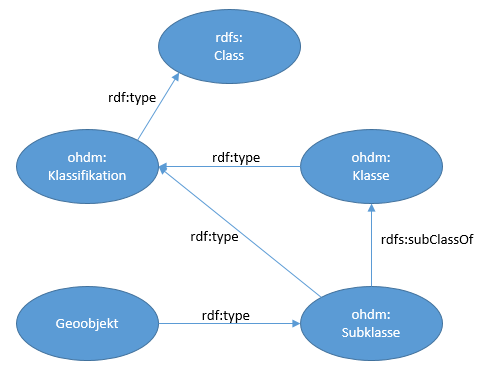
\includegraphics{sparql/ohdm-rdf.PNG}
	\caption{RDF Graph vom OHDM Modell}
	\label{fig:ohdm-rdf}
\end{figure}

\subsection{Schnittstellendefinitionen}

\subsection{genutztes Komponenten}


Den Fuseki Server kann man direkt auf der Homepage jena.apache.org runterladen (aktuelle Version 3.6.0).
Nach dem entpacken muss man den fuseki-server mit chmod die Ausführrechte geben.
Anschließend kann man dann mit ./fuseki-server den Server zum laufen bringen.
Der Server läuft dann standartmäßig auf dem Port 3030 (Portfreigabe erforderlich).
Andere Ports möglich mit ./fuseki-server --port=*number*.

Im Verzeichnis run/ in der Datei shiro.ini kann man die Rechte vergeben.
Standart User, die nicht erstellt werden müssen, sind anon und localhostFilter.
Um die Rechte für jeden Nutzer zu setzen muss man anon bearbeiten.
Um lokal die Rechte zu vergeben bearbeitet man localhostFilter.
Zusätzlich kann man unter [users] eigene Nutzer mit Passwort setzen, den man dann auch Rechte vergeben.

Für die Verbindung zur Datenbank wurde den PostGreSQL Treiber Version 42.1.4 benutz. Die im SQL-Abfrage enthaltene Daten wurden extrahiert und in einem RDF-Modell als Statement hinzugefügt.\newline

Wir haben das Apache Jena Version 3.6.0 benutzt, um RDF-Modelle zu erstellen, zu verwalten und in Dateien zu speichern. Apache Jena ist ein Java-Framework, das umfassende Bibliotheken anbietet mit denen man sehr leicht semantische Anwendungen entwickeln kann.\newline
Mit der SPARQL Bibliothek kann man direkt die RDF Datei abfragen und die Ergebnis anzeigen lassen.

\begin{figure}
	\centering
		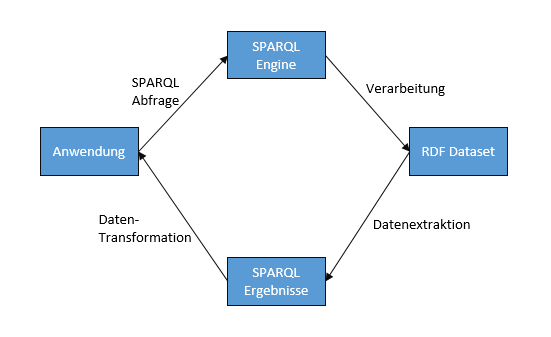
\includegraphics{sparql/sparql-abfrage.PNG}
		\caption{SPARQL Abfrage}
	\label{fig:sparql-abfrage}
\end{figure}

\section{Nutzung}
\subsection{Code}
Der Code befindet sich im SPARQL Repository.

\subsection{Deployment / Runtime}


\section{Qualitätssicherung}


\subsection{Test}


\section{Vorschläge / Ausblick}




\chapter{GeoSPARQL Schnittstelle}
\section{Dokumentengeschichte}
\begin{table}[h]
 \begin{tabular}{|l|l|p{4cm}|}
 \hline
 Zeitraum & PL/Autor(en) & Änderungen \\
 \hline
 Sommersemester 1980 & IHR NAME & 
text \newline 
text \newline 
text \newline 
text \newline 
text \newline 
text \newline 
 
  \\
 \hline
 Wintersemester 1980/81 & IHR NAME & 
text \newline 
text \newline 
text \newline 
text \newline 
text \newline 
text \newline 
 
  \\
 \hline
 \end{tabular}
 \caption{Dokumentengeschichte}
 \end{table}

\section{Aufgabe der Komponente}
Verbale kurze prägnante Beschreibung, was die Komponente leisten soll.
Das sind wenige Seiten.

(Ausfüllen in Prototyp-Phase)

\section{Architektur}

\subsection{Überlick}
Grafik der Teile der Komponente (wichtig: Benennung aller Schnittstellen). 
Anwendung der Komponente nennen (Use Case).

Übliche Interaktionen durch Interaktionsdiagramme.

(Ausfüllen in Prototyp-Phase)

\subsection{Schnittstellendefinitionen}
Beschreibung der angebotenen Schnittstellen. Benennung der Funktionen
mit Vor- und Nachbedingungen. Beschreibuung des Protocol-Bindings.

(Beginnen in Prototyp-Phase. Konkretisieren in der Alphaphase)

\subsection{genutztes Komponenten}
Beschreibung, welche weiteren Komponenten (in welchen Versionen, wo beziehbar) genutzt werden.

(Beginnen in Prototyp-Phase. Konkretisieren in der Alphaphase)

\section{Nutzung}
\subsection{Code}
Wo findet man den Code. Struktur des Codes. (In Prototyphase ausfüllen,
kann dort sehr kurz sein. Ab Alpha-Phase konkret beschreiben.)

\subsection{Deployment / Runtime}
Beschreibung wie die Komponenten aus dem Quellcode erzeugt werden kann,
wie sie installiert wird und wie man sie startet.

\section{Qualitätssicherung}
(Ausfüllen ab Alpha-Phase).

Wie erfolgt die Sicherung der Qualität? Keine Romane, sondern ehrlich notieren,
was man tut. Wenn man nichts tut, dann steht hier: Wir sichern die Qualität der
Komponente nicht.

Issue-Tracking: wie erfolgt das, interne Fehlermeldungen (ab Alpha), 
externe Fehlermeldungen ab Beta.

\subsection{Test}
Wie wird die Komponente getestet.

\section{Vorschläge / Ausblick}
Was ist aufgefallen, was sollte man ändern? Löschen Sie auch gern die Kommentare
der Vorgänger, aber nur, wenn es wirklich nicht mehr relevant ist.



\chapter{Data Provenance}
\section{Dokumentengeschichte}
\begin{table}[h]
 \begin{tabular}{|l|l|p{4cm}|}
 \hline
 Zeitraum & PL/Autor(en) & Änderungen \\
 \hline
 Sommersemester 1980 & IHR NAME & 
text \newline 
text \newline 
text \newline 
text \newline 
text \newline 
text \newline 
 
  \\
 \hline
 Wintersemester 1980/81 & IHR NAME & 
text \newline 
text \newline 
text \newline 
text \newline 
text \newline 
text \newline 
 
  \\
 \hline
 \end{tabular}
 \caption{Dokumentengeschichte}
 \end{table}

\section{Aufgabe der Komponente}
Verbale kurze prägnante Beschreibung, was die Komponente leisten soll.
Das sind wenige Seiten.

(Ausfüllen in Prototyp-Phase)

\section{Architektur}

\subsection{Überlick}
Grafik der Teile der Komponente (wichtig: Benennung aller Schnittstellen). 
Anwendung der Komponente nennen (Use Case).

Übliche Interaktionen durch Interaktionsdiagramme.

(Ausfüllen in Prototyp-Phase)

\subsection{Schnittstellendefinitionen}
Beschreibung der angebotenen Schnittstellen. Benennung der Funktionen
mit Vor- und Nachbedingungen. Beschreibuung des Protocol-Bindings.

(Beginnen in Prototyp-Phase. Konkretisieren in der Alphaphase)

\subsection{genutztes Komponenten}
Beschreibung, welche weiteren Komponenten (in welchen Versionen, wo beziehbar) genutzt werden.

(Beginnen in Prototyp-Phase. Konkretisieren in der Alphaphase)

\section{Nutzung}
\subsection{Code}
Wo findet man den Code. Struktur des Codes. (In Prototyphase ausfüllen,
kann dort sehr kurz sein. Ab Alpha-Phase konkret beschreiben.)

\subsection{Deployment / Runtime}
Beschreibung wie die Komponenten aus dem Quellcode erzeugt werden kann,
wie sie installiert wird und wie man sie startet.

\section{Qualitätssicherung}
(Ausfüllen ab Alpha-Phase).

Wie erfolgt die Sicherung der Qualität? Keine Romane, sondern ehrlich notieren,
was man tut. Wenn man nichts tut, dann steht hier: Wir sichern die Qualität der
Komponente nicht.

Issue-Tracking: wie erfolgt das, interne Fehlermeldungen (ab Alpha), 
externe Fehlermeldungen ab Beta.

\subsection{Test}
Wie wird die Komponente getestet.

\section{Vorschläge / Ausblick}
Was ist aufgefallen, was sollte man ändern? Löschen Sie auch gern die Kommentare
der Vorgänger, aber nur, wenn es wirklich nicht mehr relevant ist.



\chapter{CIDOC CRM Unterstützung}
\section{Dokumentengeschichte}
\begin{table}[h]
 \begin{tabular}{|l|l|p{4cm}|}
 \hline
 Zeitraum & PL/Autor(en) & Änderungen \\
 \hline
 Sommersemester 1980 & IHR NAME & 
text \newline 
text \newline 
text \newline 
text \newline 
text \newline 
text \newline 
 
  \\
 \hline
 Wintersemester 1980/81 & IHR NAME & 
text \newline 
text \newline 
text \newline 
text \newline 
text \newline 
text \newline 
 
  \\
 \hline
 \end{tabular}
 \caption{Dokumentengeschichte}
 \end{table}

\section{Aufgabe der Komponente}
Verbale kurze prägnante Beschreibung, was die Komponente leisten soll.
Das sind wenige Seiten.

(Ausfüllen in Prototyp-Phase)

\section{Architektur}

\subsection{Überlick}
Grafik der Teile der Komponente (wichtig: Benennung aller Schnittstellen). 
Anwendung der Komponente nennen (Use Case).

Übliche Interaktionen durch Interaktionsdiagramme.

(Ausfüllen in Prototyp-Phase)

\subsection{Schnittstellendefinitionen}
Beschreibung der angebotenen Schnittstellen. Benennung der Funktionen
mit Vor- und Nachbedingungen. Beschreibuung des Protocol-Bindings.

(Beginnen in Prototyp-Phase. Konkretisieren in der Alphaphase)

\subsection{genutztes Komponenten}
Beschreibung, welche weiteren Komponenten (in welchen Versionen, wo beziehbar) genutzt werden.

(Beginnen in Prototyp-Phase. Konkretisieren in der Alphaphase)

\section{Nutzung}
\subsection{Code}
Wo findet man den Code. Struktur des Codes. (In Prototyphase ausfüllen,
kann dort sehr kurz sein. Ab Alpha-Phase konkret beschreiben.)

\subsection{Deployment / Runtime}
Beschreibung wie die Komponenten aus dem Quellcode erzeugt werden kann,
wie sie installiert wird und wie man sie startet.

\section{Qualitätssicherung}
(Ausfüllen ab Alpha-Phase).

Wie erfolgt die Sicherung der Qualität? Keine Romane, sondern ehrlich notieren,
was man tut. Wenn man nichts tut, dann steht hier: Wir sichern die Qualität der
Komponente nicht.

Issue-Tracking: wie erfolgt das, interne Fehlermeldungen (ab Alpha), 
externe Fehlermeldungen ab Beta.

\subsection{Test}
Wie wird die Komponente getestet.

\section{Vorschläge / Ausblick}
Was ist aufgefallen, was sollte man ändern? Löschen Sie auch gern die Kommentare
der Vorgänger, aber nur, wenn es wirklich nicht mehr relevant ist.



\chapter{OHDM OfflineMaps mit Xamarin}
\section{Dokumentengeschichte}
\begin{table}[h]
 \begin{tabular}{|l|l|p{4cm}|}
 \hline
 Zeitraum & PL/Autor(en) & Änderungen \\
 \hline
 Sommersemester 2017 & Schulz, Daniel & 
Kapitel erstellt und Software dokumentiert \newline  
  \\
 \hline
 \end{tabular}
 \caption{Dokumentengeschichte}
 \end{table}

\section{Aufgabe der Komponente}

Bei den OHDM OfflineMaps (oder auch der OHDMApp) mit Xamarin handelt es sich um eine mobile Anwendung, welche vorab einen Datenexport aus OHDM erhält und danach in der Lage ist auf dem mobilen Gerät offline die entsprechenden Karten zu einem selbst bestimmbaren Zeitpunkt zu rendern.
So kann in der App beispielsweise der 01.02.1790 ausgewählt werden und es würden die zu diesem Datum gültigen Kartendaten dargestellt werden.
Da die Anwendung auf Xamarin und C\# basiert kann sie jederzeit mit geringem Aufwand auch auf iOS portiert und ausgerollt werden. (Bisher wird nur Android unterstützt)

\section{Architektur}

\subsection{Überlick}\label{ch:offlineoverview}

\hspace*{-3em}
\includegraphics*[width=1.3\linewidth,natwidth=1137,natheight=1042]{offlinemaps/bilder/komponentendiagramm.png}

In der obenstehenden durch Visual Studio automatisiert generierten CodeMap lassen sich die einzelnen Bestandteile der Xamarin-Anwendung ablesen, sowie die extern eingebundenen Bibliotheken/NuGet-Pakete.\\
\newpage
Nachfolgend werden alle Bestandteile sehr kurz erläutert:\\
\\
\begin{itemize}
	\item MainActivity: Diese Klasse ist für das UserInterface unter Android zuständig und definiert jegliche Interaktion mit dem Benutzer.
	\item MapDrawer: Diese Klasse definiert die grundlegende Darstellung von Kartenelementen, also zum Beispiel in welchen Zoomstufen sie gerendert werden und welche Styles sie nutzen.
	\item CsvUtils: Diese Klasse beinhaltet die Implementierung der Übertragung der Kartendaten aus einer CSV, welche zuvor aus der OHDM-Datenbank erzeugt wurde in eine neue interne SQLite-Datenbank für die Anwendung.
	\item MapEventHandler, MapEventArgs, CsvEventHandler, CsvEventArgs: Diese Klassen definieren Events, welche bei den verschiedenen Datenverarbeitungsschritten der App genutzt werden um dem Anwender den Fortschritt zu signalisieren.
	\item Styles: In dieser Klasse werden die Styles definiert, welche der MapDrawer später anwendet. Dies sind zum Beispiel die Farbe und Stärke von Linien, Punkten oder Polygonen.
	\item DatabaseHelper: Der DatabaseHelper definiert die Schnittstellen und Funktionen zur Anbindung an die lokale SQLite-Datenbank, welche zur Datenhaltung der eingelesenen Kartendaten genutzt wird.
	\item PostgisObjectMap: Diese Klasse wird genutzt um die Felder der PostgisObjects auf die Spalten der Daten-CSV zu mappen.
	\item PostgisObject, PostgisPoint, PostgisPolygon, PostgisLine: Diese Klassen stellen die objektbasierte Darstellung der Daten aus der OHDM-Datenbank dar, welche vom Programm genutzt wird.
	\item GlobalData: Diese Klasse ist nur eine statische Klasse zur Zwischenspeicherung von Daten auf welche von mehreren Klassen zugegriffen werden muss von denen nicht alle den nötigen Kontext aufweisen.
\end{itemize}
\newpage
Nachfolgend werden alle externen Libraries erläutert, welche nicht automatisiert von Xamarin geladen oder benötigt werden, sondern spezifisch für die Anwendung erforderlich sind:\\
\\
\begin{itemize}
	\item CartoMobileSDK: Hierbei handelt es sich um das Karten-Framework Carto, welches zur Darstellung der Offline-Karten genutzt wird.\\ \url{https://carto.com/docs/carto-engine/mobile-sdk/}
	\item CsvHelper: Bei CsvHelper handelt es sich um ein .NET basiertes Framework zum automatisierten einlesen und mappen von Objekten aus einer CSV-Datei.\\
	\url{https://github.com/JoshClose/CsvHelper}
	\item Newtonsoft.JSON: Hierbei handelt es sich um ein Framework zur Serialisierung und Deserialisierung von Objekten in JSON-Objekte.\\
	\url{https://www.newtonsoft.com/json}
	\item SQLite-net: Hierbei handelt es sich um eine Multiplattform-Bibliothek, welche die Erzeugung und Anbindung von SQLite-Datenbanken ermöglicht.\\
	\url{https://github.com/praeclarum/sqlite-net}
\end{itemize}

\subsection{Schnittstellendefinitionen}\label{ch:offlineinterfaces}
Die einzige Quasi-Schnittstelle, welche von den OfflineMaps genutzt bzw. benötigt wird ist ein Datenexport mit OHDM-Daten aus einer OHDM-Datenbank.
Zum Einlesen wird ein CSV-File in der folgenden Struktur benötigt:\\
\begin{lstlisting}[
basicstyle=\footnotesize
]
id;name;type_target;classification_id;classname;subclassname;valid_since;
valid_until;point;line;polygon
19;"S Tiergarten";1;396;"public_transport";"stop_position";"2015-12-22";
"2017-07-10";"{""type"":""Point"",""coordinates"":[13.3364598,52.5142085]}";"";""
20;"S Tiergarten";1;542;"railway";"station";"2015-12-22";
"2017-07-10";"{""type"":""Point"",""coordinates"":[13.3364598,52.5142085]}";"";""
65;"Jakob-Kaiser-Platz";1;589;"highway";"motorway_junction";"2017-01-01";
"2017-07-10";"{""type"":""Point"",""coordinates"":[13.2906741,52.533132]}";"";""
112;"S Pichelsberg";1;542;"railway";"station";"2016-03-04";
"2017-07-10";"{""type"":""Point"",""coordinates"":[13.2275633,52.5102387]}";"";""
136;"S Schoeneberg";1;583;"highway";"bus_stop";"2016-03-11";
"2017-07-10";"{""type"":""Point"",""coordinates"":[13.3529104,52.4797246]}";"";""
\end{lstlisting}
\newpage
Aus der Berliner-OHDM-Datenbank, welche auf dem PostgreSQL-Server der HTW Berlin liegt können die Daten in diesem Format mit der folgenden Abfrage extrahiert werden:

\begin{lstlisting}[
basicstyle=\footnotesize
]
SELECT gog.id, go.name, gog.type_target, gog.classification_id, 
c.class as classname, c.subclassname, gog.valid_since, gog.valid_until, 
ST_AsGeoJSON(p.point) as point, ST_AsGeoJSON(l.line) as line, 
ST_AsGeoJSON(poly.polygon) as polygon

FROM berlin.geoobject as go, berlin.classification as c, berlin.geoobject_geometry as gog

LEFT OUTER JOIN berlin.points as p ON gog.type_target=1 AND gog.id_target=p.id

LEFT OUTER JOIN berlin.lines as l ON gog.type_target=2 AND gog.id_target=l.id

LEFT OUTER JOIN berlin.polygons as poly ON gog.type_target=3 AND gog.id_target=poly.id

WHERE go.id=gog.id_geoobject_source AND gog.classification_id=c.id AND 
gog.type_target>0 AND gog.type_target<4 AND 
(point IS NOT NULL OR line IS NOT NULL OR polygon IS NOT NULL);
\end{lstlisting}

Alternativ könnten die Daten auch aus den Rendering-Tabellen bezogen werden, hierzu müsste nur eine neue Abfrage entwickelt werden und das Programm von WGS84, welches bisher genutzt wird, auf Pseudo-Mercator umgestellt werden.

\subsection{Genutzte Komponenten}

In der Anwendung wurden die folgenden Komponenten, welche zuvor in Kapitel \ref{ch:offlineoverview} detaillierter beschrieben wurden in den angegebenen Versionen benutzt:\\
\\
\begin{itemize}
	\item CartoMobileSDK: Version 4.1.0
	\item CsvHelper: Version 2.16.3.0\\(Achtung! Diese Version ist wichtig, da in der nachfolgenden Version die Nutzung komplett umgestellt wurde und ein komplettes Rewrite des CSV-Codes erfordern würde.)
	\item Newtonsoft.JSON: Version 10.0.3
	\item SQLite-net bzw. sqlite-net-pcl: Version 1.4.118 
\end{itemize}
Alle Versionen können ganz normal über den in Visual Studio integrierten NuGet-Paketmanager installiert werden.
\newpage
\section{Nutzung}
\subsection{Code}
Der aktuelle Code kann unter\\ \url{https://github.com/OpenHistoricalDataMap/OfflineMaps}\\ bezogen werden. Die Struktur des Codes wurde bereits in Kapitel \ref{ch:offlineoverview} erläutert und grafisch dargestellt.

\subsection{Deployment / Runtime}
Als Vorbedingung für das Deployment müssen zuerst folgende Dinge auf dem PC, welcher eingesetzt werden soll vorliegen bzw. installiert sein:\\
\\\\
Android ADB-Treiber von dem Mobilgerät, auf welchem später die Anwendung deployed werden soll.\\
Der Standard-Google-Treiber kann hier bezogen werden:\\ \url{https://developer.android.com/studio/run/win-usb.html}\\
Alternativ sind noch diese möglich: \url{https://adb.clockworkmod.com}\\
Hierbei ist zu beachten, dass jeder Gerätehersteller zum Teil eigene Treiber benötigt, vor allem Samsung, diese sind separat im Internet zu beziehen.\\\\
Zusätzlich muss das USB-Debugging auf Android aktiviert werden, wie hier beschrieben:\\
\url{https://www.howtogeek.com/129728/how-to-access-the-developer-options-menu-and-enable-usb-debugging-on-android-4.2/}\\\\\\
Es muss ein Datenextrakt aus der OHDM-Datenbank in Form einer CSV-Datei vorliegen. In Kapitel \ref{ch:offlineinterfaces} wird erläutert, wie und in welchem Format dieser zu erzeugen ist.\\ Die Datei muss hinterher den Namen ``outputnew.csv'' erhalten.\\\\\\
Um das OfflineMaps-Projekt zu bearbeiten oder zu deployen ist als Entwicklungsumgebung Visual Studio 2017 mit Xamarin nötig.\\
Visual Studio 2017 kann theoretisch in der kostenlosen Community-Edition heruntergeladen und installiert werden, da aber für Hochschulangehöroge die Enterprise-Version über Microsoft Imagine/Dreamspark kostenlos bezogen werden kann, sollte diese genutzt werden und in der nachfolgenden Erläuterung wird auch nur auf diese eingegangen.\\
Informationen zum Download von Microsoft-Produkten für Hochschulangehörige der HTW Berlin finden sich hier:\\
\url{http://www.f4.htw-berlin.de/studieren/softwarelizenzen/}\\
Im nachfolgenden Link wird erläutert mit welchen Optionen Visual Studio 2017 installiert werden muss um Xamarin-Projekte zu unterstützen:\\
\url{https://developer.xamarin.com/guides/cross-platform/getting_started/installation/windows/}\\
Die Xamarin-Installation entsprechend dem Guide ist zwingend erforderlich!
Zusätzlich müssen im Installationsbildschirm von Visual Studio 2017, in welchem auch die Xamarin-Pakete angehakt werden auch zwingend alle Git und GitHub-Pakete, sowie Pakete, welche das Android SDK betreffen angehakt werden, hierzu sollten alle Unterpunkte durchgeklickt und durchsucht werden.\\\\
Nachdem Visual Studio 2017 mit allen zuvor beschriebenen Komponenten installiert wurde, kann es gestartet werden.\\
Anschließend kann man dem Tutorial von Microsoft zum Klonen eines Git-Repos ab dem Punkt ``Clone from another Git Provider'' folgen (die Punkte darüber können ignoriert werden):\\
\url{https://docs.microsoft.com/en-us/vsts/git/tutorial/clone?tabs=visual-studio#clone-from-another-git-provider}\\
Der Git-Link des Repos der OfflineMaps, welcher zum klonen eingesetzt wird lautet: 
\url{https://github.com/OpenHistoricalDataMap/OfflineMaps.git}\\
Gegebenfalls fragt VisualStudio vor dem Klonen noch die eigenen GitHub-Zugangsdaten ab.\\\\
Nachdem die Solution entsprechend der Angaben des Microsoft-Tutorials geklont und geöffnet wurde ist das Projekt nahezu bereit zum Deployment und es müssen nur noch zwei individuelle Schritte ausgeführt werden:\\\\
Zuerst muss in der AndroidManifest.xml, welche sich unter Properties befindet ein eigener Name für das Package gesetzt werden, da es sonst später zu Fehlern mit dem API-Key kommt.\\
In der Klasse MainActivity muss die Stringkonstante LICENSE in welcher nur exemplarisch ``XXX'' steht gegen einen eigenen API-Key von Carto ausgetauscht werden. Dieser kann von Carto kostenlos erzeugt werden gemäß der nachfolgenden Anleitung unter dem Punkt ``Registering your App'':\\
\url{https://carto.com/docs/carto-engine/mobile-sdk/getting-started/#registering-your-app}\\\\
Als letzten Schritt muss nur noch die im Projektverzeichnis unter Assets liegende ``outputnew.csv'' durch die ausgetauscht werden, welche gemäß Kapitel \ref{ch:offlineinterfaces} erzeugt wurde.\\\\
Danach kann die App durch einen Klick auf den grünen Pfeil im oberen Zentrum der Navigationsleisten oder einen Druck auf F5 auf dem (an den PC angeschlossenen) Android-Gerät deployed und ausgeführt werden.\\
Sollte es Fehlermeldungen wegen nicht korrekt geladener NuGet-Pakete geben, so können diese in der NuGet-Konsole (Extras -> NuGet-Paket-Manager -> Paket-Manager-Konsole) mit dem Befehl ``update-package -reinstall'' neu initialisiert werden.\\\\
Zusätzlicher Hinweis: Durch einen Bug im aktuellen Android-SDK verhält sich Android Oreo noch etwas seltsam, so schließt sich beim Ausführen über Visual Studio die Anwendung direkt wieder. Hier muss die Anwendung nachdem sie über Visual Studio installiert wurde einfach vom Handy aus gestartet werden, dann funktioniert alles. Für das Debugging sollte aus diesem Grund aktuell Android in der Version  $\leq7.1.2$ verwendet werden. Außerdem ist dringend anzuraten, alle Visual Studio und Android SDK Updates zu installieren.


\section{Qualitätssicherung}

Die Qualitätssicherung der Darstellung erfolgt bisher durch akribische Abgleiche der OHDM-Darstellung mit der aktuellen deutschen OSM-Darstellung und die Angleichung an dieselbe. Für das Handling der Anwendung was Verständlichkeit und Performance angeht wurde die Qualität durch externe unbeteiligte Personen bewertet und dann verbessert.\\
\\
Issue-Tracking: Bisher keines.

\subsection{Test}
Die Komponente kann momentan ausschließlich durch Anwender-Testgruppen getestet werden und nicht automatisiert, aufgrund der Komplexität der Darstellung. Es wäre allenfalls möglich die Datenimport und -Exportfunktionen um Unit-Tests zu erweitern, was aber aktuell noch nicht umgesetzt ist. 

\section{Vorschläge / Ausblick}
In der Anwendung sind bisher nur exemplarisch die wichtigsten Typen an OSM-Objekten mit spezifischen Rendering-Merkmalen für eine spezifische Darstellung versehen. Hier bietet es sich an auch die übrigen zu implementieren. Außerdem wäre es sinnvoll und gewinnbringend die vorhandene Xamarin-Codebasis zu erweitern und um die entsprechenden iOS und UWP-Schnittstellen zu erweitern um die Anwendung auch auf iOS- und Windows-Geräten zum Einsatz bringen zu können.

\end{document}
